\newpage
\section{Conditional branching (full title)}
\genHeader
\hypertarget{sec:conBran}{}

{\bf \large this is appendix content. Be sure to review to make sure it flows with the document.}

When working with SDMs, you often need to choose between two different patterns based on the return value of an arbitrary (black box) operation.
This is like the normal \texttt{Success}/\texttt{Failure} construction, but instead of a pattern being matched or failing, the decision can be implemented with
a another SDM or a standard Java method. This feature is a further means (besides \texttt{MethodCallExpressions} for attribute values and \texttt{Bindings}) of
integrating hand-written Java code in SDMs (and can lead to spaghetti SDMs so please use with caution!).

As an example, consider a class \texttt{A} with an operation:
\begin{quote}
 \mbox{\texttt{doSomeCheck(p$_1$,\ldots,p$_n$ :EClass) :EBoolean}}
\end{quote}

This method could be implemented in hand-written Java code or be specified by another SDM specification.

Although dummy boolean attributes \emph{could} be used to achieve the same effect, it is much simpler to branch the control flow based on the result of a \texttt{StatementNode}.
If the method returns an \texttt{EBoolean}, \texttt{Success} and \texttt{Failure} correspond to \texttt{true} and \texttt{false}, respectively. If the method returns anything else, then \texttt{Failure} corresponds to \texttt{null}. Void methods \emph{cannot} be used to branch and an exception is thrown during code generation.

Figure~\ref{fig:cond_branch_on_op} depicts the class \texttt{A}, and shows how \texttt{doSomeCheck} is used to branch in an SDM.

\begin{figure}[htp]
\begin{center}
  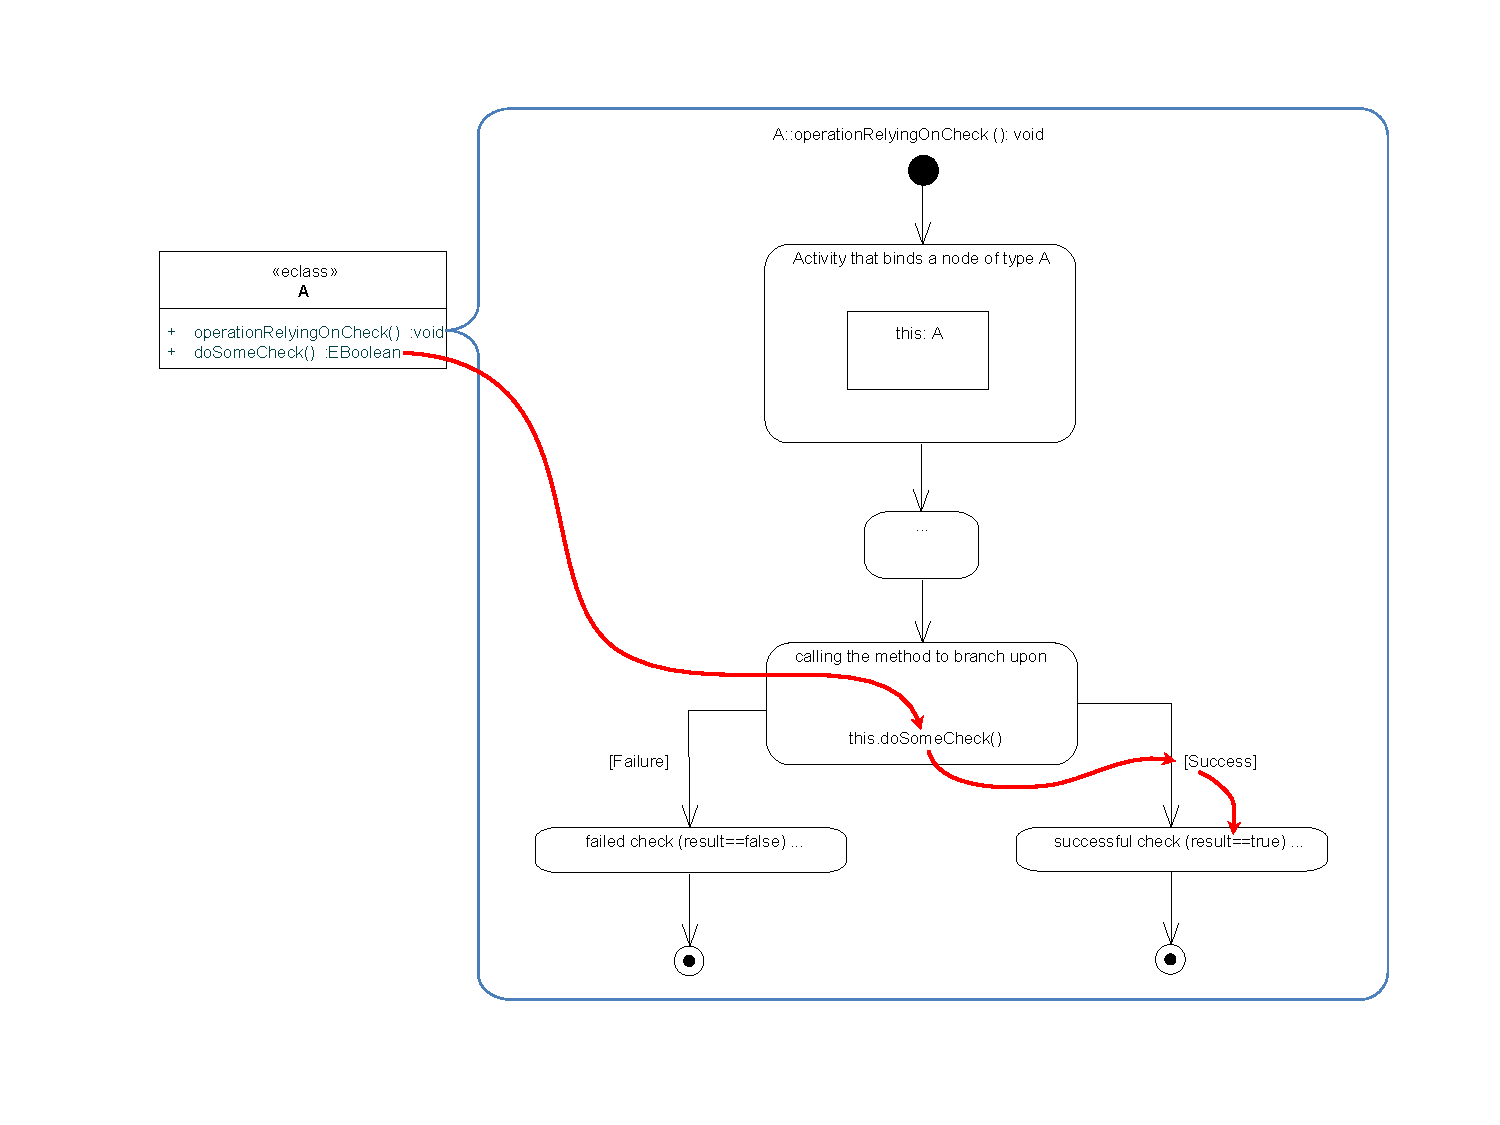
\includegraphics[width=1.0\textwidth]{SDM_with_branch}
  \caption{Conditional branching based on the result of an operation}
  \label{fig:cond_branch_on_op}
\end{center}
\end{figure}

\vspace{0.5cm}
\begin{itemize}
\item[$\blacktriangleright$] As always, click on a link below to begin.
\end{itemize}

\begin{center} {$\triangleright$ \hyperlink{conBran vis}{Conditional Branching: The visual syntax}}%
\\ \vspace{0.5cm}
 {$\triangleright$ \hyperlink{conBran tex}{Conditional Branching: The textual syntax}}\end{center} 

\clearpage
\hypertarget{conBran vis}{}
\subsection{Branching with statement nodes}
\visHeader

\begin{itemize}
  
\item[$\blacktriangleright$] Edit the \texttt{Box} class in your metamodel by invoking the \texttt{Operations} dialogue and create a new method called
\texttt{initalizeBox}. Recalling the sole condition of conditional branching, set its return type to \texttt{EBoolean}. Save the method, then re-open the
\texttt{grow} SDM.

\vspace{0.5cm}

\item[$\blacktriangleright$] Add a new \texttt{StatementNode} from \texttt{addNewPartitionBox} and name it \texttt{initialize}. The edge guard should
automatically set itself to \texttt{failure}.

\vspace{0.5cm}

\item[$\blacktriangleright$] In the \texttt{Statement} tab, invoke a \texttt{MethodCallExpression} to your new method.

\vspace{0.5cm}

\item[$\blacktriangleright$] Finally, attach two \texttt{StopNode}s -- \texttt{true} and \texttt{false} -- along with their appropriate edge guards. These mean
that the if method call succeeds, the box could be initialized, so it will return a literal \texttt{true}. If it failed however, \texttt{box} was already in an
invalid state (by, i.e., having only one card) and returns \texttt{false}. Overall, the new additions to \texttt{box.grow()} should resemble
Fig.~\ref{fig:newGrowControl}.

\vspace{0.5cm}

\begin{figure}[htp]
\begin{center}
  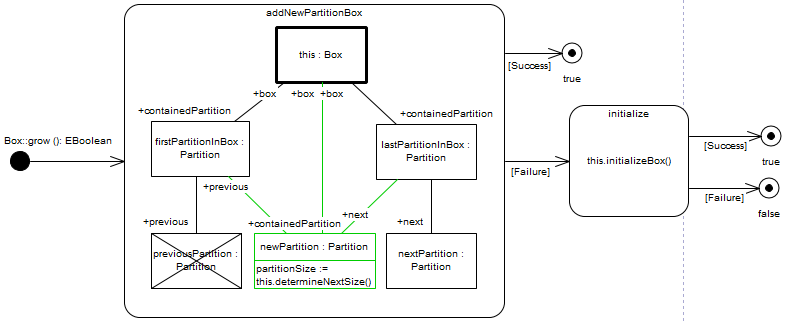
\includegraphics[width=\textwidth]{ea_growAdditions}
  \caption{Extending \texttt{grow} with a \emph{MethodCallExpression}}
  \label{fig:newGrowControl}
\end{center}
\end{figure}

\clearpage

\item[$\blacktriangleright$] Switch back to your open \texttt{Box.grow} SDM in EA. You'll notice that if you double-click on \texttt{initialize}, the
\texttt{Extract Story Pattern} option is invalid. This makes sense -- you don't define a pattern in a statement node. Instead, return to the main diagram and
create a new SDM for \texttt{initializeBox}.

\item[$\blacktriangleright$] In its diagram, create an \texttt{activity node} named \texttt{buildPartitions}. Within it, have a bound \texttt{Box} linked to a
\texttt{onePartition} NAC, and two other `green' (create) object variables, \texttt{firstPartition} and \texttt{lastPartition}. Be sure to also connect two
true/false \texttt{StopNode}s. The pattern should now resemble Fig.~\ref{fig:buildPartitions}. The NAC here can only fulfilled if the box has no partitions,
i.e., is in a pristine state and able to be initialized. In other words, If \texttt{grow} is used for an empty box, it initializes the box for the first time
and grows it after that, ensuring that the box is always in a valid state.

\vspace{0.5cm}
 
\begin{figure}[htp]
\begin{center}
  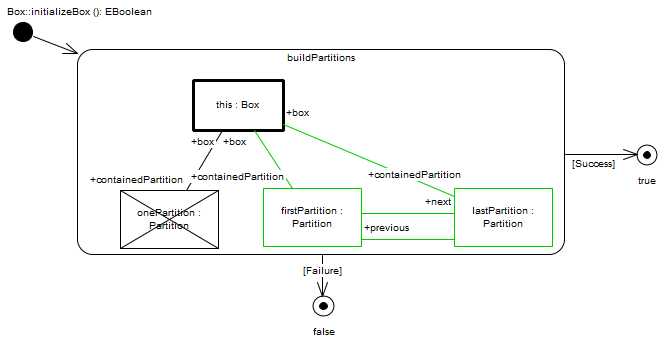
\includegraphics[width=\textwidth]{eclipse_buildPartitions}
  \caption{Compelted NAC to check for \emph{one} partition}
  \label{fig:buildPartitions}
\end{center}
\end{figure}
 
\item[$\blacktriangleright$] You're finished! Save, validate, and build your metamodel, then check out how this is done in the textual syntax in
Fig.~\ref{fig:updateGrow} and Fig.~\ref{fig:pattBuildParts}.

\jumpSingle{initialize notes}

\end{itemize}


\newpage
\hypertarget{conBran tex}{}
\subsection{Branching with statement nodes}
\texHeader

\begin{itemize}

\item[$\blacktriangleright$] Before doing anything else, let's declare the method that will insert two new partitions into \texttt{box} when the original
pattern match fails. Open \texttt{Box.eclass} and add the following signature anywhere in the file: 
\syntax{initializeBox() : EBoolean}

\vspace{0.5cm}

\item[$\blacktriangleright$] Now modify \texttt{Box.grow()} by adding a nested \emph{if/Else} construct, with \texttt{[addNewPartitionBox]} as the
first conditional, and execute a \emph{statement node} if it fails. \texttt{grow} should now resemble Fig.~\ref{fig:updateGrow}.

\vspace{0.5cm}

\begin{figure}[htp]
\begin{center}
  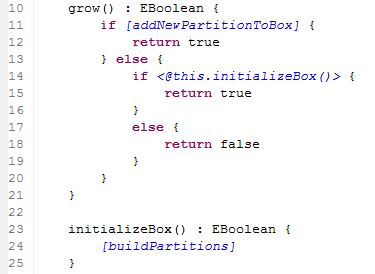
\includegraphics[width=0.5\textwidth]{eclipse_updateGrow}
  \caption{Extending \texttt{Box} with a \emph{statement node}}
  \label{fig:updateGrow}
\end{center}
\end{figure}

\vspace{0.5cm}

\item[$\blacktriangleright$] Next, we want to specify our newest method. Create a new pattern called \texttt{buildPartitions} in its scope. Complete
the pattern as illustrated in Fig.~\ref{fig:pattBuildParts}.

\item[$\blacktriangleright$] As you can see, we have created a NAC that can only be fulfilled if the box has no lonely partition. In turn, this means that if a
box is completely empty, it will be intialized for the first time with two partitions, and guaranteed to remain in a valid state if growing continues.

\clearpage

\vspace*{2cm}

\begin{figure}[htp]
\begin{center}
  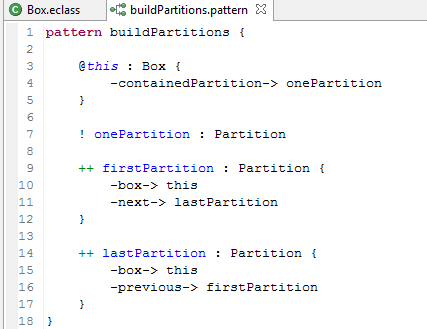
\includegraphics[width=0.7\textwidth]{eclipse_buildPartitionsPattern}
  \caption{NAC initalizing an empty box}
  \label{fig:pattBuildParts}
\end{center}
\end{figure}

\item[$\blacktriangleright$] That's it! Save and build your metamodel to make sure no errors exist. To see how this is depicted in the visual syntax, check out
Fig.~\ref{fig:newGrowControl} and Fig.~\ref{fig:buildPartitions}.

\end{itemize}
